\documentclass{article}
\textheight 22.5truecm \textwidth 14.5truecm
\setlength{\oddsidemargin}{0.35in}\setlength{\evensidemargin}{0.35in}

\usepackage[utf8]{inputenc}
\usepackage[russian]{babel}
\usepackage{graphicx}
\usepackage{amsmath}
\usepackage{breqn}
\usepackage{wrapfig}
\usepackage{float}
\usepackage{multirow}
\usepackage{caption}
\usepackage{subcaption}

\graphicspath{ {./data/images} }
\author{Александр Романов Б01-110}
\date{}
\title{1.3 Изучение рассеяния медленных электронов на атомах (эффект Рамзауэра)}

\begin{document}
\maketitle
\section{Введение}
\subsection{О работе}
Исследуется энергетическая зависимость вероятности рассеяния электронов атомами ксенона, определяются
энергии электронов, при которых наблюдается "просветление" ксенона, и оцениваетчя размер его внешней
электронной оболочки.

\begin{figure}[H]
	\centering
	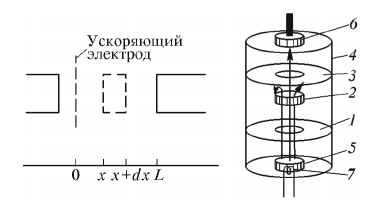
\includegraphics[width=0.6\textwidth]{scheme.png}
	\caption{Схематическое изображение тиратрона (слева) и его конструкция (справа): 
	1, 2, 3 -- сетки; 4 -- внешний металлический циллиндр; 5 -- катод; 6 -- анод;
	7 -- накаливаемая спираль}
\end{figure}

\section{Работа}
Включив все приборы переведём осциллограф в режим внешней развёртки и установим
напряжение накала на уровень \(2.5\;V\). Пронаблюдаем картину вольт-амперной
характеристики эффекта Рамзауэра.

\begin{figure}[H]
	\centering
	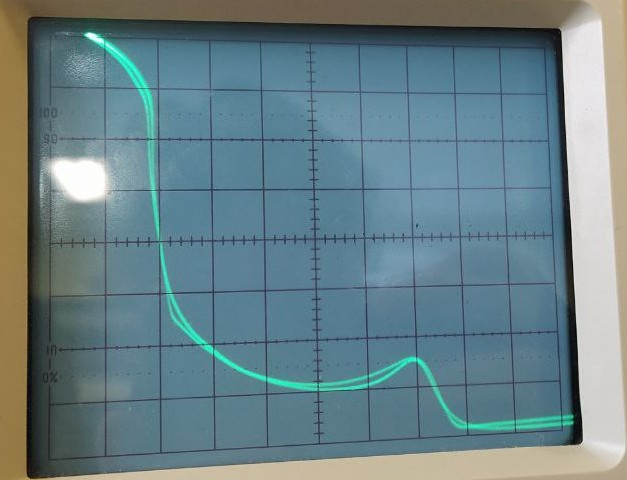
\includegraphics[width=0.6\textwidth]{signal.jpeg}
	\caption{ВАХ эффекта Рамзауэра}
\end{figure}

На изображении отчётливо видны максимумы и минимумы (Отметим что развёртка производится
справа налево).

Проведём расчёт размера электронной оболочки атома инертного газа, заполняющего лампу:

\[ R = \frac{1}{2}\frac{h}{\sqrt{2m(E_1 + U_0)}} = (3.07 \pm 0.05)\;10^{-10}m  \]

Также вычислим глубину потенциальной ямы исходя из данных с осциллографа для двух значений
напряжения накала.
\(V = 2.56\;V\):
\[ U_0 = \frac{4}{5}E_2 - \frac{9}{5}E_1 = 2.00 \pm 0.005 \;V\]
\(V = 2.93\;V\):
\[ U_0 = \frac{4}{5}E_2 - \frac{9}{5}E_1 = 1.56 \pm 0.005\;V\]

Запишем значения напряжения пробоя. \(U_b = 18.6 \pm 0.1\;eV\) для \(U_h = 2.56\;V\) и
\(U_b = 18.6 \pm 0.1\;eV\) для \(U_h = 2.93\;V\). Полученные значения свопадают друг с другом
и лучше всего соотносятся с таковым значением для аргона (\(15.6\;eV\))

Проведём измерения ВАХ тиратрона в статическом режиме установки для двух значений
напряжения накала: \(2.53\;V\) и \(2.97\;V\). Результаты занесём в таблицу и построим графики:

\begin{table}[H]
\centering
\begin{tabular}{|c|c|}
\hline
V, V & I, mA      \\\hline
0.513   & 0.062 \\\hline
1       & 0.651  \\\hline
1.15    & 0.994  \\\hline
1.25    & 1.167  \\\hline
1.5     & 1.446  \\\hline
1.6     & 1.570   \\\hline
1.75    & 1.615  \\\hline
1.8     & 1.613  \\\hline
2       & 1.498  \\\hline
2.5     & 1.197  \\\hline
3       & 0.923  \\\hline
3.5     & 0.762  \\\hline
3.99    & 0.665  \\\hline
4.5     & 0.591 \\\hline
5       & 0.550   \\\hline
5.51    & 0.523  \\\hline
6       & 0.523  \\\hline
6.5     & 0.541  \\\hline
7       & 0.551  \\\hline
7.5     & 0.567  \\\hline
8       & 0.586  \\\hline
8.5     & 0.641  \\\hline
9       & 0.706  \\\hline
9.51    & 0.814  \\\hline
10      & 0.892 \\\hline
10.5    & 0.963  \\\hline
11      & 0.109   \\\hline
11.5    & 1.322  \\\hline
11.9    & 1.432  \\\hline
\end{tabular}
	\caption{\(2.53V\)}
\end{table}

\begin{table}[H]
\centering
\begin{tabular}{|c|c|}
\hline
V\_c, V & I, A   \\\hline
0.126   & 0.0055 \\\hline
0.254   & 0.0247 \\\hline
0.379   & 0.0654 \\\hline
0.497   & 0.1342 \\\hline
0.627   & 0.265  \\\hline
0.75    & 0.4565 \\\hline
0.875   & 0.6958 \\\hline
0.992   & 0.951  \\\hline
1.125   & 1.218  \\\hline
1.245   & 1.417  \\\hline
1.37    & 1.574  \\\hline
1.5     & 1.672  \\\hline
1.63    & 1.726  \\\hline
1.75    & 1.7395 \\\hline
1.873   & 1.7265 \\\hline
2       & 1.694  \\\hline
2.12    & 1.65   \\\hline
2.222   & 1.609  \\\hline
2.378   & 1.543  \\\hline
2.4     & 1.531  \\\hline
2.6     & 1.452  \\\hline
2.8     & 1.38   \\\hline
3       & 1.322  \\\hline
3.21    & 1.274  \\\hline
3.398   & 1.239  \\\hline
3.587   & 1.21   \\\hline
3.8     & 1.187  \\\hline
4       & 1.168  \\\hline
4.2     & 1.15   \\\hline
4.51    & 1.133  \\\hline
5       & 1.134  \\\hline
5.5     & 1.137  \\\hline
6       & 1.18   \\\hline
6.5     & 1.243  \\\hline
6.99    & 1.312  \\\hline
7.5     & 1.403  \\\hline
8.02    & 1.52   \\\hline
8.511   & 1.65   \\\hline
9       & 1.813  \\\hline
9.5     & 2.08   \\\hline
10      & 2.3    \\\hline
10.6    & 2.6    \\\hline
11.07   & 2.9    \\\hline
11.5    & 3.3    \\\hline
11.5    & 3.3    \\\hline
\end{tabular}
\caption{\(2.97\;V\)}
\end{table}

\section{Выводы}
\end{document}
